\section{Efficient Action Tokenization via Time-Series Compression}
\label{sec:method} 



\begin{figure*}[t]
    \centering
    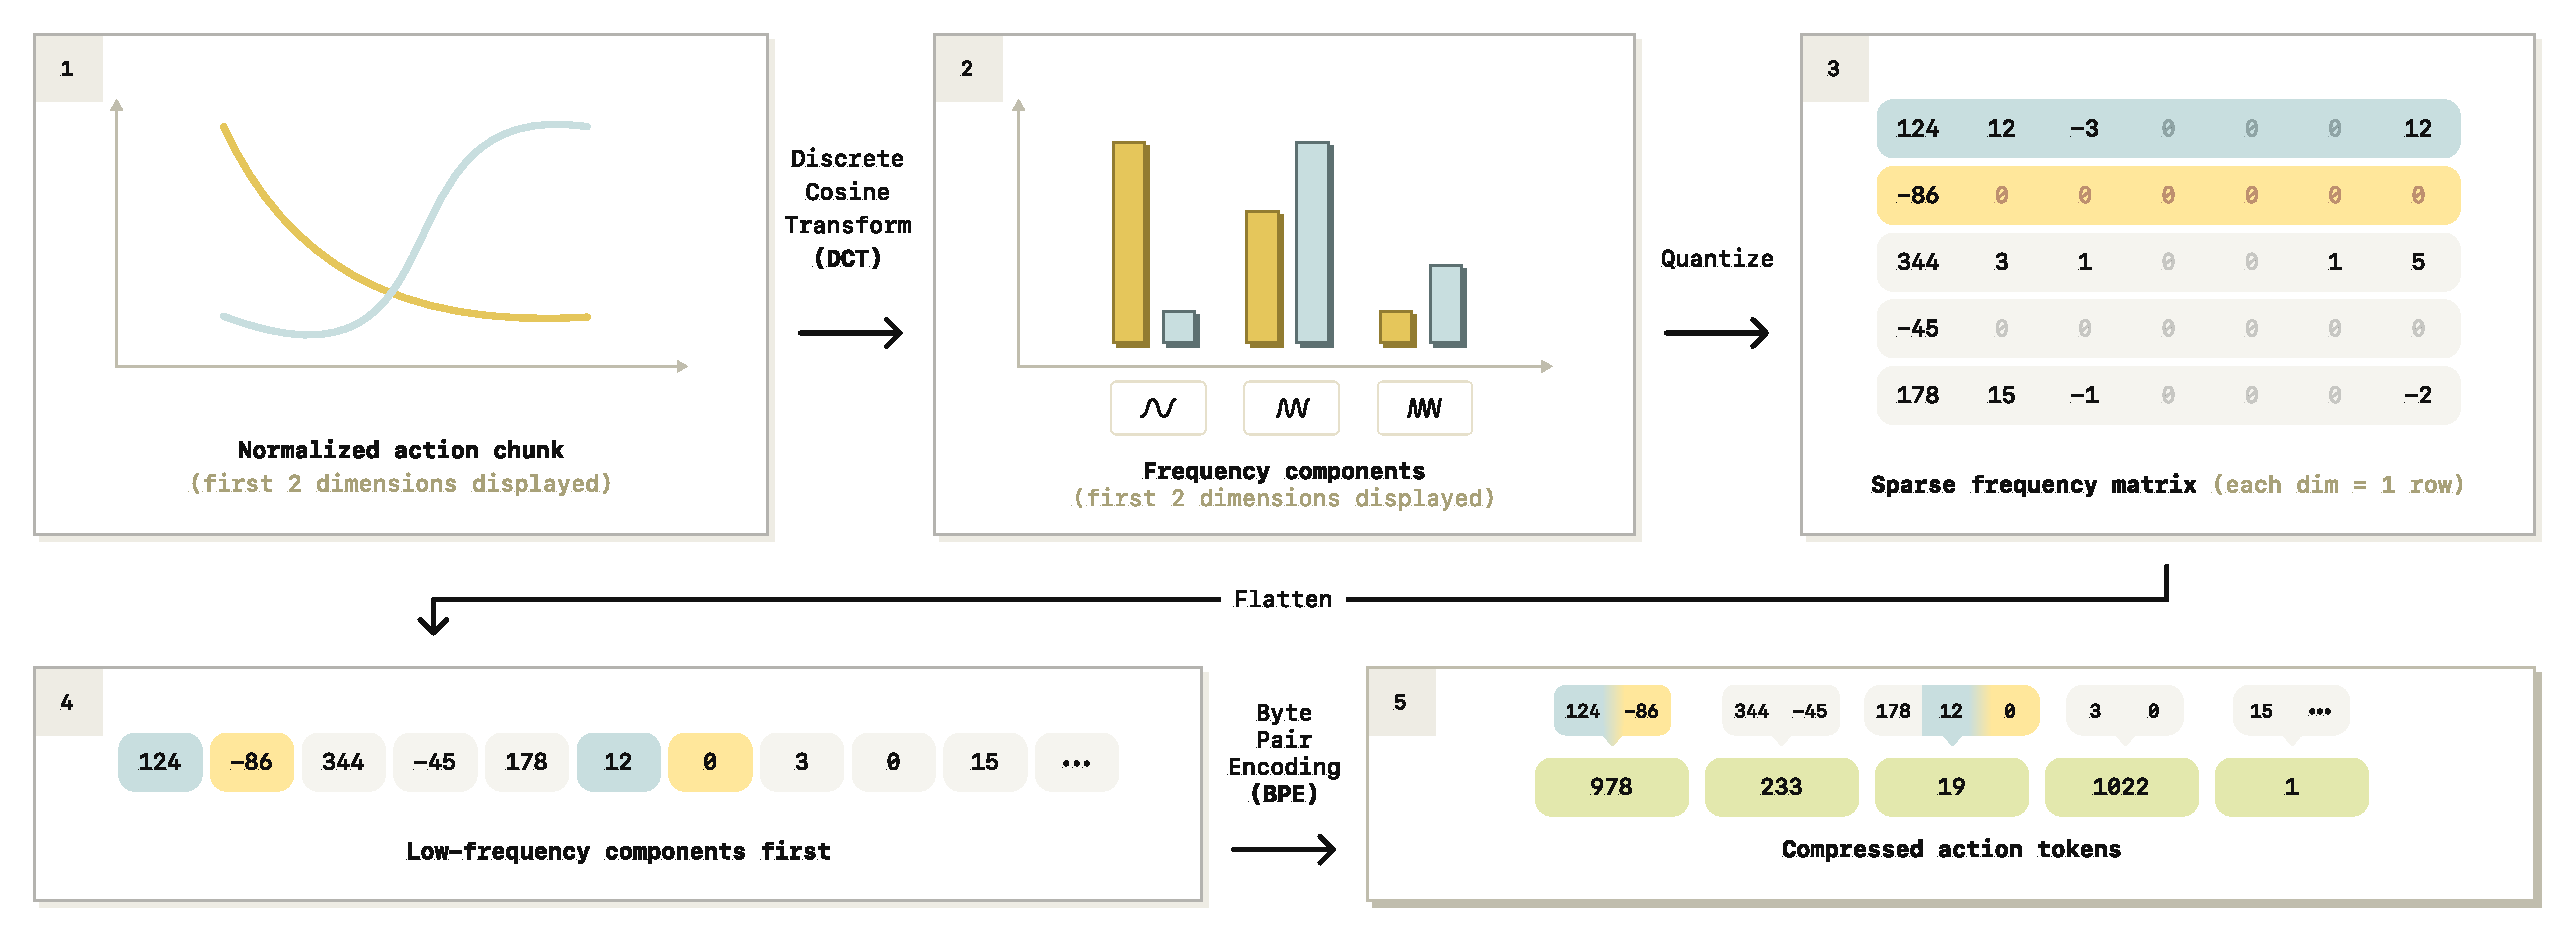
\includegraphics[width=\linewidth]{figures/dct_method.pdf}
    \caption{\textbf{Overview of the \ModelAcronym~action tokenization pipeline.} Given a normalized chunk of actions, we apply discrete cosine transform (DCT) to convert the signal to the frequency domain. We then quantize the DCT coefficients and use byte-pair encoding (BPE) to compress the flattened sequence of per-dimension DCT coefficients into the final action token sequence. See \cref{sec:dct_tokenizer} for a detailed description.}
    \label{fig:method_overview}
\end{figure*}

We saw in the previous section how redundancy in high-frequency action trajectories can lead to low marginal information for each action token, and thereby poor training performance. To address this, we need a tokenization approach that compresses the highly redundant action signal into a smaller number of high-information tokens. In this section, we will first describe a simple approach for compressing continuous time series (\ref{sec:dct}), then use it to design an action tokenization algorithm (\cref{sec:dct_tokenizer}), and finally explain how we train a \emph{universal} tokenizer for robot actions (\cref{sec:universal_tokenizer}).

\subsection{Time-Series Compression via Discrete Cosine Transform}
\label{sec:dct}

There is a rich body of work on effectively compressing continuous time series, from approaches that compress signals after transforming them into the frequency domain \citep{fft, dct, jpeg} to \emph{learned} compression approaches, e.g., based on vector quantization~\cite{vqvae,fsq}. One key takeaway of our work is that \emph{any} sufficiently effective compression approach, when applied to the action targets, is suited to improve the training speed of VLA models. In practice, there are a few considerations that may still lead us to favor some compression algorithms over others, e.g., the complexity of training the tokenizer, and how efficient is it at tokenizing and detokenizing actions.

In this work, we use a compression algorithm based on the discrete cosine transform (DCT)~\cite{dct}. DCT is a frequency-space transform that represents a continuous signal as a sum of cosine elements of various frequencies. Low frequencies capture the overall shape of the signal, while high-frequency components reflect sharp jumps. DCT is a commonly used transformation for compression algorithms, e.g., for JPEG image compression~\citep{jpeg}, due to its simplicity and computational efficiency, and its strong compression property on practical images: since pixels often vary smoothly, DCT can often represent most of the information of an input signal in only a few coefficients. Signals can be compressed by omitting frequency components with low weights. Compared to learned compression approaches based on vector quantization, DCT-based compression is an analytical approach, thus extremely simple and fast.


\subsection{The \ModelAcronym~Tokenization Algorithm}
\label{sec:dct_tokenizer}

We use the discrete cosine transform to design \ModelAcronym, a quick and effective tokenization approach for robot actions. We detail the steps from raw robot actions to action tokens in \cref{fig:method_overview}. We first normalize the input actions, such that the 1st and 99th quantile of values in the training dataset for each action dimension maps to the range $[-1, \dots, 1]$. This initial normalization step is useful to bring the data into a specified range and also makes tokenization of cross-embodied datasets with different action scales easier. We use quantiles to be robust to outlier actions which occasionally occur in large robot datasets. After the data is normalized, we apply the discrete cosine transform to each action dimension separately. To compress the DCT-converted signal we can simply omit insignificant coefficients, which we implement through a scale-and-round operation, where the scaling coefficient is a hyperparameter that trades off between lossiness and compression rate of the tokenization operation.

After the rounding operation, the DCT coefficient matrix is typically sparse, with most entries being zero and only a few significant coefficients remaining per action dimension. To actually realize the compression, we must convert this sparse matrix into a sequence of dense tokens. We flatten the matrix into a 1-dimensional vector of integers, interleaving action dimensions by including all low-frequency components first, and train a byte pair encoding (BPE) tokenizer~\citep{gage1994new} to losslessly compress it into dense action tokens. The BPE step ``squashes'' the zero-valued components and merges frequently-occurring coefficient combinations across action dimensions. We choose BPE to compress the DCT matrix, since many efficient implementations exist and it can produce a fixed-size output vocabulary that can be easily integrated into the existing vocabulary of vision-language models for VLA training. Other lossless compression algorithms like Huffman coding~\citep{huffmancode} or Lempel-Ziv methods~\citep{lempelziv} (the algorithms underlying the gzip compression approach) could be used instead, but we leave this investigation for future work.

Note that the \emph{order} of flattening the $\vert A \vert \times H$ DCT coefficient matrix prior to BPE encoding can have significant impact on policy training. There are two options: column-first flattening, i.e., concatenate the lowest-frequency components for each dimension first, or row-first flattening, i.e., concatenating all frequency components for a single action dimension first. We choose the former, since we find that predicting the \emph{low-frequency} components, that characterize the overall shape of the output sequence, first during autoregressive prediction leads to more stable policy rollouts.

\begin{algorithm}[t]

\caption{\ModelAcronym~Tokenizer}
\label{alg:fast}
\begin{algorithmic}
\Require scale $\gamma$, (for inference) BPE dictionary $\Phi$
\Procedure{FASTTokenizer}{$a_{1:H}$}
    \State $C^i_{j} \gets \texttt{DCT}\left(a^{i}_{1:H}\right)$ \Comment{Compute DCT coefficients}
    \State $\bar C^i_{j} \gets \texttt{round}\left(\gamma \cdot C^i_{j}\right)$ \Comment{Quantize coefficients}
    \State $\left[T_k\right] \gets \left[\bar C^1_1, \bar C^2_1, \dots, C^1_2, \dots, C^n_H\right]$ \Comment{Flatten tokens}

\noindent \textbf{BPE Training}:
    \State $\phi \gets \texttt{TrainBPE}(\mathcal{D} := \{[T_k]\})$

\noindent \textbf{Tokenization}:
    \State $\left[{\bar T}_1, \dots, {\bar T}_{\bar k}\right] \gets \texttt{BPE}\left([T_1, \dots, T_k], \phi\right)$
    \State \Return $\text{action\_tokens}$
\EndProcedure
\end{algorithmic}
\end{algorithm}

All operations in our tokenization pipeline are easily invertible, allowing fast decoding of predicted actions. The tokenizer has only two hyperparameters: the scale applied to the DCT coefficients before rounding, and the vocabulary size of the BPE compression step. We find that both parameters are not very sensitive, and we use the same values across all our single-dataset tokenization experiments (rounding scale 10, BPE vocabulary size 1024). This is in contrast to end-to-end \emph{learned} compression modules that rely on vector quantization~\cite{vqvae}. Such networks are often tedious to train, and require careful dataset-specific hyperparameter selection to achieve good reconstruction~\cite{yu2023magvit,fsq}. Our experiments show that our DCT-based tokenization approach trains higher-performing policies than VQ-based approaches, while being significantly simpler and easier to tune. %

We empirically demonstrate the benefits of our DCT-based tokenization in the toy example from \cref{sec:educational_example}. \cref{fig:toy_example} shows that training the autoregressive model on DCT-compressed target tokens achieves constantly low prediction error across a wide range of sampling frequencies. We provide a concise summary of our tokenization approach in \cref{alg:fast} and test the effectiveness of \ModelAcronym~tokenization on robot control problems in \cref{sec:experiments}. 


\subsection{A Universal Robot Action Tokenizer}
\label{sec:universal_tokenizer}

The only \emph{learned} component of our tokenizer is the vocabulary of the BPE encoder, which needs to be trained for each new dataset that the tokenizer is being applied to. While this learning process is fast (typically only a few minutes), it adds additional friction to using \ModelAcronym~tokenization. Thus, we aim to train a \textbf{universal} action tokenizer, that can encode chunks of robot actions from \emph{any} robot. To this end, we train a tokenizer using the pipeline described above on a large, cross-embodied robot action dataset, consisting of approximately one million 1-second action chunks from single-arm, bi-manual and mobile manipulation robots, with joint and end-effector control action spaces and various control frequencies. We provide a detailed breakdown of the data mixture used for training the universal tokenizer in \cref{sec:app_universal_data_mix}. Once trained, our universal action tokenizer, \ModelUniversalAcronym, can be applied as a black-box tokenizer on 1-second action sequences from any robot setup. Our experimental evaluation shows that it is competitive to tokenizers tuned for individual datasets. 

\noindent\textbf{Code release.} We release our pre-trained universal action tokenizer, \ModelUniversalAcronym, in a convenient HuggingFace \texttt{AutoProcessor} class, that makes it easy to apply the tokenizer to any new robot action chunk in three lines of code:


\lstset{
  language=Python,
  basicstyle=\ttfamily\small,
  keywordstyle=[1]\color{green!50!black}\bfseries,   %
  keywordstyle=[2]\color{blue}\bfseries,   %
  commentstyle=\color{grey},                      %
  stringstyle=\color{red!70!black},               %
  identifierstyle=\color{black},       %
  showstringspaces=false,
}

\begin{lstlisting}[language=Python]
from transformers import AutoProcessor

tokenizer = AutoProcessor.from_pretrained(
    "physical-intelligence/fast", 
    trust_remote_code=True
)
tokens = tokenizer(action_chunk)
\end{lstlisting}

For best compression results, we recommend normalizing input actions to range $[-1, \dots, 1]$ via quantile normalization as described in \cref{sec:dct_tokenizer}, and tokenizing 1-second action chunks at a time. 
Our module also makes it easy to train a \emph{new} \ModelAcronym~tokenizer on a given dataset of action chunks:
\begin{lstlisting}[language=Python]
from transformers import AutoProcessor

tokenizer = AutoProcessor.from_pretrained(
    "physical-intelligence/fast", 
    trust_remote_code=True
)
new_tokenizer = tokenizer.fit(action_dataset)
\end{lstlisting}





